\section{Mô hình ngôn ngữ lớn - LLMs}
\subsection{Tổng quan về LLMs}
Mô hình ngôn ngữ lớn (LLMs) là nền tảng quan trọng của các hệ thống NLP hiện đại, đóng vai trò mô hình cốt lõi cho các ứng dụng trí tuệ nhân tạo tạo sinh. Các mô hình này được xây dựng từ mạng nơ-ron sâu với số lượng tham số rất lớn, thường từ hàng trăm triệu đến hàng trăm tỷ, cho phép chúng học ngữ cảnh và mô hình hoá ngôn ngữ hiệu quả trên các tập dữ liệu văn bản quy mô lớn. Nhờ đó, LLMs thể hiện khả năng linh hoạt trong nhiều tác vụ như sinh văn bản, tóm tắt, dịch thuật, trả lời câu hỏi hay suy luận ở mức độ nhất định.

Sự phát triển của LLMs gắn liền với kiến trúc Transformer, được đề xuất trong công trình “Attention Is All You Need” (Vaswani et al., 2017). Transformer có khả năng mô hình hoá quan hệ phụ thuộc dài hạn và hỗ trợ xử lý song song, vượt trội so với RNN/LSTM. Các mô hình hiện đại như GPT, Claude hay Gemini đều dựa trên kiến trúc này.
% \cite{vaswani2017attention} .

\begin{figure}
    \centering
    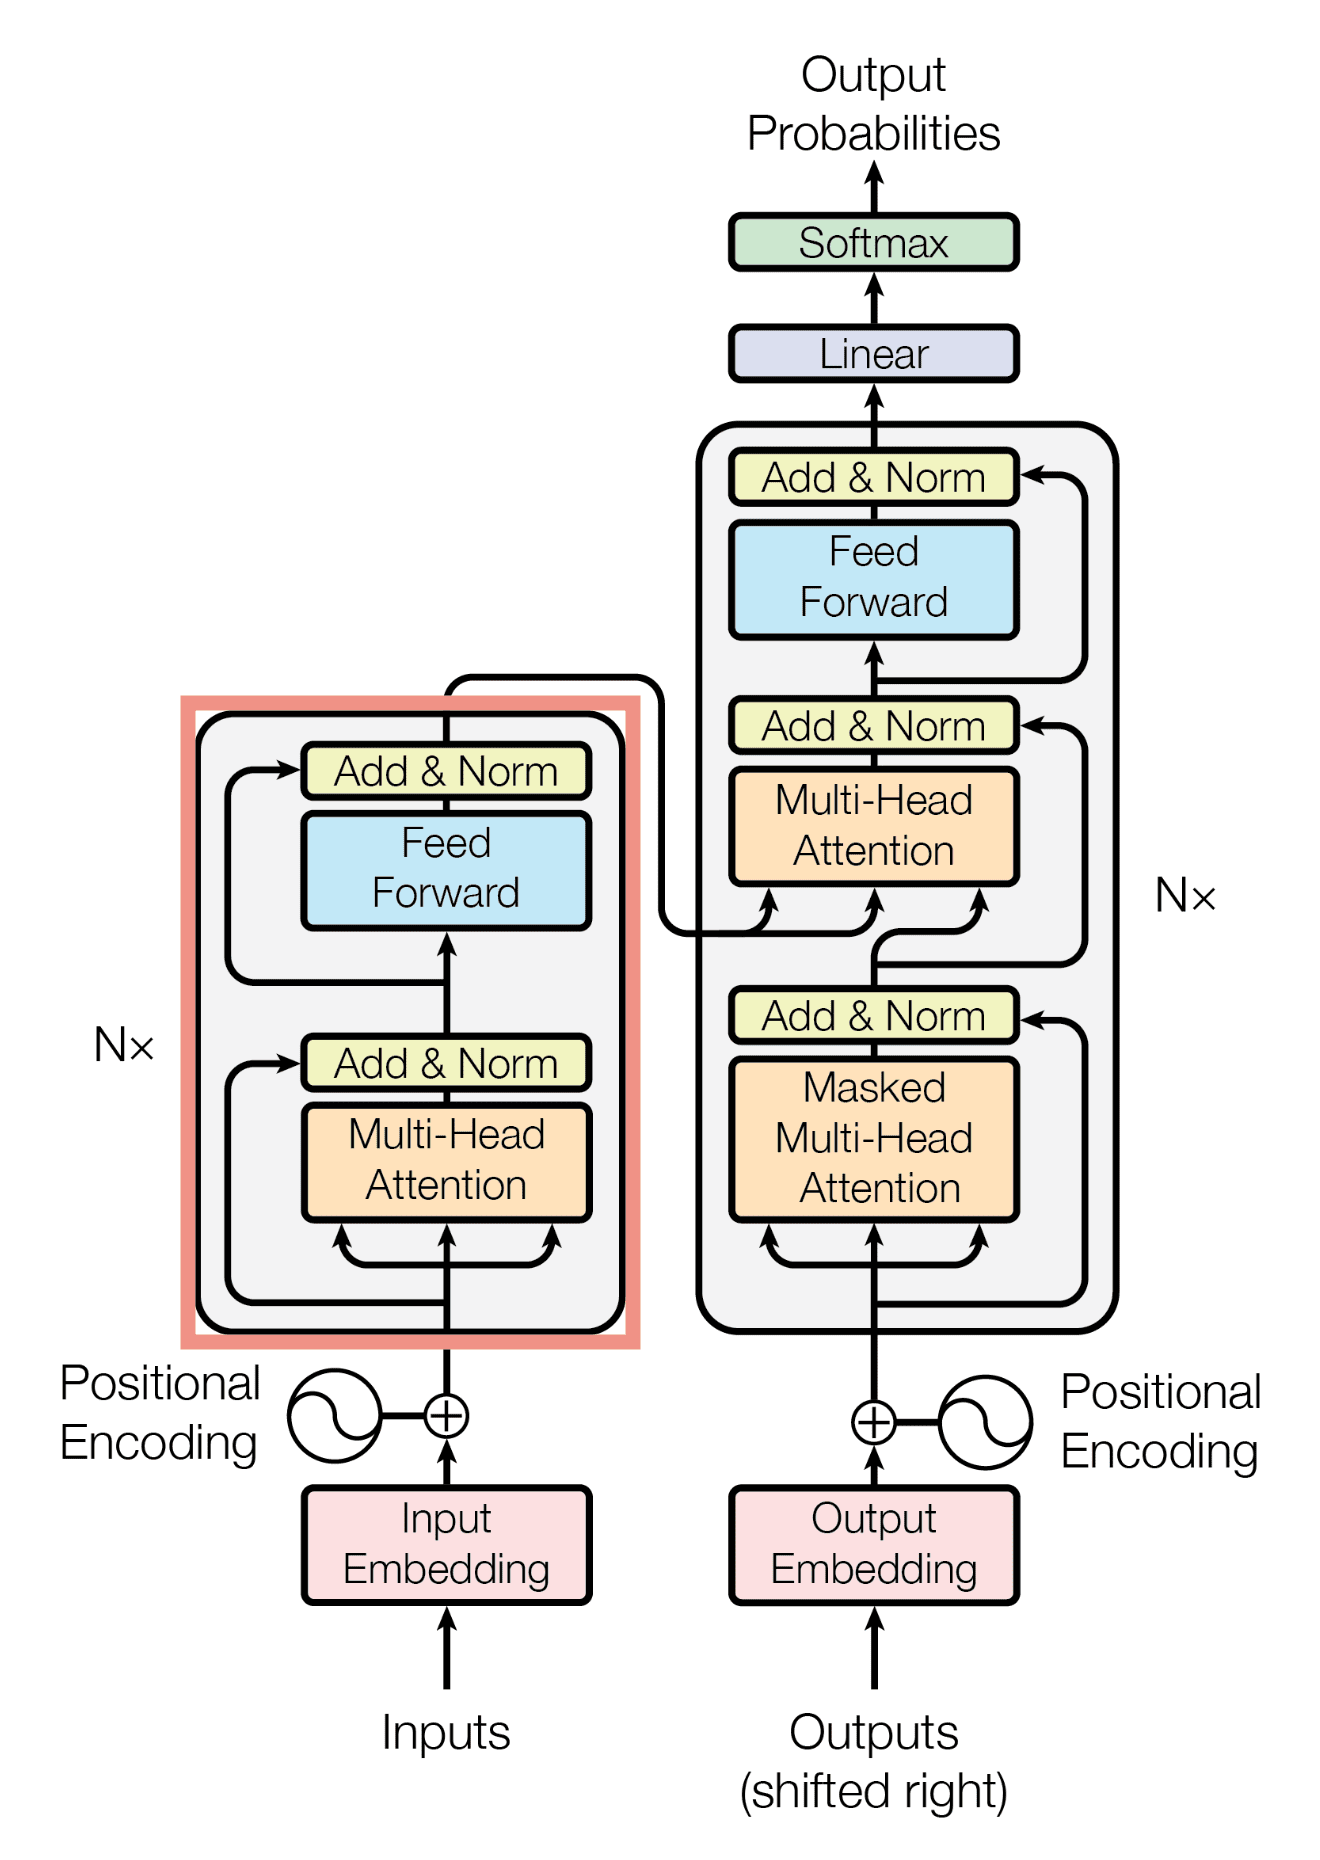
\includegraphics[width=0.25\linewidth]{figures/transformer_1.png}
    \caption{The Transformer - model architecture. Source: %\cite{vaswani2017attention}
    }
    \label{fig:Transformer}
\end{figure}

Hình~\ref{fig:Transformer} minh hoạ kiến trúc Transformer với hai thành phần chính: \textit{encoder} và \textit{decoder}, mỗi khối gồm cơ chế \textit{multi-head self-attention}, mạng \textit{feed-forward} và các kết nối tắt kèm chuẩn hoá lớp, tạo nền tảng cho khả năng học quan hệ phụ thuộc dài hạn và xử lý song song.

\subsection{Kiến trúc và cơ chế hoạt động của LLMs}

Mô hình ngôn ngữ lớn (Large Language Models -- LLMs) hiện là nền tảng cốt lõi của hầu hết các hệ thống xử lý ngôn ngữ tự nhiên và trí tuệ nhân tạo tạo sinh hiện đại. Các mô hình này được xây dựng dựa trên kiến trúc Transformer \cite{vaswani2017attention}, bao gồm hàng trăm triệu đến hàng nghìn tỷ tham số, cho phép học biểu diễn ngữ nghĩa phong phú từ các tập dữ liệu văn bản quy mô cực lớn.

Trong giai đoạn tiền huấn luyện (pre-training), LLMs được huấn luyện theo phương pháp self-supervised learning với các mục tiêu chính như causal language modeling hoặc masked language modeling\cite{devlin2019bert, radford2019language, brown2020language}. Nhờ đó, mô hình không chỉ nắm bắt cấu trúc ngữ pháp và đặc trưng ngôn ngữ mà còn lưu trữ một lượng tri thức thực tế khổng lồ dưới dạng parametric knowledge, giúp chúng thực hiện hiệu quả nhiều tác vụ như trả lời câu hỏi, tóm tắt, dịch thuật và suy luận nhỏ mà không cần huấn luyện bổ sung đáng kể \cite{bommasani2021opportunities}.

Một đặc trưng quan trọng của LLMs là khả năng học ngữ cảnh (in-context learning) \cite{brown2020language}. Chỉ cần cung cấp vài ví dụ hoặc hướng dẫn chi tiết trong prompt (zero-shot hoặc few-shot prompting), mô hình có thể nhanh chóng thích nghi với định dạng đầu ra mong muốn, chẳng hạn phong cách học thuật, cách trình bày niên đại chính xác, hoặc phân biệt rõ ràng giữa sự kiện đã xác minh và giả thuyết lịch sử. Khả năng này đặc biệt có giá trị trong các ứng dụng hỏi–đáp lịch sử đòi hỏi tuân thủ nghiêm ngặt yêu cầu chuyên môn.

Tuy nhiên, khi áp dụng trực tiếp vào lĩnh vực lịch sử, hai hạn chế lớn của cơ chế hoạt động hiện tại đã bộc lộ rõ:

\begin{enumerate}
    \item \textbf{Tri thức tĩnh}: Mô hình chỉ phản ánh dữ liệu huấn luyện đến một thời điểm cắt nhất định (training data cut-off), do đó không thể tự cập nhật các phát hiện mới, tài liệu giải mật gần đây, các hướng giải thích lịch sử đương đại hoặc đơn giản là các thay đổi lịch sử vừa được đính chính.\cite{lazaridou2021mind}.
    \item \textbf{Ảo giác (hallucination)}: LLMs thường sinh ra thông tin sai lệch hoặc không tồn tại (niên đại sai, nhầm lẫn sự kiện, bịa đặt chi tiết) nhưng trình bày với độ tự tin cao \cite{ji2023survey}. Các bộ đánh giá như TruthfulQA \cite{lin2021truthfulqa}, HaluEval \cite{li2023halueval} và HALO \cite{zhang2023hallucination} cho thấy tỷ lệ hallucination vẫn đáng kể, đặc biệt với các câu hỏi yêu cầu tri thức chuyên sâu hoặc suy luận đa bước.
\end{enumerate}

Để khắc phục, các phương pháp tinh chỉnh hiệu quả về tham số như LoRA \cite{hu2022lora}, QLoRA \cite{dettmers2023qlora}, DoRA \cite{liu2024dora} đã được phát triển, cho phép thích nghi mô hình với dữ liệu lịch sử chuyên biệt (sử liệu tiếng Việt, văn bản cổ, thuật ngữ chuyên ngành) chỉ bằng cách điều chỉnh một phần rất nhỏ trọng số gốc, đồng thời bảo toàn tri thức tổng quát.

Mặc dù vậy, ngay cả sau khi tinh chỉnh, LLMs vẫn gặp khó khăn khi xử lý ngữ cảnh dài và thực hiện suy luận đa bước phức tạp -- vốn là yêu cầu xuất hiện nhiều trong nghiên cứu lịch sử. Do đó, trong các hệ thống hỏi–đáp lịch sử thực tế, LLMs gần như luôn được kết hợp với cơ chế truy xuất thông tin bên ngoài, tiêu biểu là Retrieval-Augmented Generation (RAG) \cite{lewis2020retrieval}, nhằm cung cấp bằng chứng cập nhật và giảm thiểu tối đa nguy cơ ảo giác.
